\documentclass[pageno]{jpaper}

\newcommand{\IWreport}{2015}

\usepackage{hyperref}
\usepackage{couriers}
\usepackage[normalem]{ulem}
\usepackage{listings}
\usepackage{lstlangcoq}
\usepackage{appendix}
\usepackage{graphicx}

\lstset{language=Coq,basicstyle=\ttfamily,mathescape=true,columns=fullflexible,breaklines=true,breakatwhitespace=true}
\hypersetup{citecolor=black,linkcolor=black}
\graphicspath{ {images/} }

\widowpenalty500
\clubpenalty500

\newcommand{\stdtitle}[1]{\textbf{#1}}

\begin{document}

\title{
Verification of a Deterministic Random Bits Generator
}

\author{Naphat Sanguansin\\Adviser: Andrew W. Appel}

\date{}
\maketitle

\thispagestyle{empty}
\doublespacing
\begin{abstract}
In this project, I formally verified the \stdtitle{mbedTLS} implementation of a HMAC-based deterministic random bits generator (DRBG) with respect to the standard \stdtitle{NIST SP 800-90A}. By “formal”, I mean the verification is in the machine-checked environment of Coq using the Verified Software Toolchain (VST) framework. I verified the functions \lstinline{update}, \lstinline{reseed}, and \lstinline{generate}. Due to time constraint, I was not able to verify the \lstinline{instantiate} function.
\end{abstract}

\section{Introduction}
A deterministic random bits generator (DRBG) is a program that takes a source of randomness, or entropy, and stretches it out into a much longer string of pseudorandom bits. \stdtitle{NIST SP 800-90A} \cite{nist} DRBG provides backtracking resistance and, optionally, prediction resistance. Backtracking resistance means that even if the whole (secret) state of the DRBG is known at time $t$, an adversary will not be able to distinguish between a truly random bitstring and a bitstring generated by the DRBG at some time before $t$. Prediction resistance is the complement, providing the same assurance for some time including and after $t$. Here, “time” is counted in terms of calls to the \lstinline{generate} function.

\stdtitle{NIST SP 800-90A} specifies different types of DRBG. The version I verified in this project is the one based on the key-hashed message authentication code, or HMAC. HMAC takes a (secret) key and a message and computes a fixed-length message authentication code. In theory, someone with only the message will not be able to compute the message authentication code, and someone with both the message and the message authentication code will not be able to compute the key. Note that HMAC is an irreversible function.

Why did I choose to verify an implementation of DRBG? In short, DRBG is a widely used crypto primitive. Correctly implemented crypto primitives help application programmers improve the security of their code without them having to fully understand the math behind the crypto algorithms.

\subsection{Machine-Checked Proofs}
I did the verification in Coq, an open-sourced proof assistant. The C code is compiled into its abstract syntax tree (AST) in Coq using the CompCert certified (proved correct with a machine-checked proof) compiler. I wrote functional specifications (functional programs) in Coq that closely match \stdtitle{NIST SP 800-90A}. Using the functional programs, I created API specifications using the VST framework. API specifications reason about how the AST deals with memory and local variables. I then proved the AST correct with respect to the API specifications.

Of what the tasks I mentioned, the ones that must be trusted are the translation of \stdtitle{NIST SP 800-90A} into functional specifications and the creation of API specifications from those functional programs. Everything else is machine-checked. Can the functional and API specifications be trusted? For the latter, I hope to make a convincing claim by the end of this paper that as long as the functional specifications are correct, the corresponding API specifications will be, too. As for the functional specifications, first of all, they are small, easy-to-reason-about, strongly typed functional programs. I also ran the programs on some test inputs from NIST and verified that the output matches. That said, it is still unsatisfying that at the functional specification level, I had to resort to unit tests. Thankfully, there is a parallel project by Katherine Ye ‘16 that will prove cryptographic properties of the functional specifications. The fact that this parallel project can be done in concurrent to (and mostly independent from) the verification of the C implementation shows the power and flexibility of VST.

\subsection{Related Works}
Similar verifications have been done for SHA-256 and HMAC, see \cite{sha} and \cite{hmac} respectively. As mentioned previously, Katherine Ye ‘16 is working on proving cryptographic properties of the functional specifications.

As far as I could tell, this is the first end-to-end verification of an implementation of HMAC DRBG against a functional specification. By “end-to-end” I mean that the verification builds upon an existing verification of HMAC \cite{hmac} (which is, in turn, built upon an existing verification of SHA-256 \cite{sha}).

There have been some other verification efforts to verify a DRBG, albeit without using a functional specification. As an example, D{\"o}rre and Klebanov \cite{prng} verified Android’s pseudorandom number generator. This verification is done on a Java implementation, and is a verification on information flow, not on a functional specification. That is, the project proves that all the bytes of entropy are used in constructing the secret internal state, but not \textit{how} the bytes are used. Proving an implementation against a functional specification is arguably better, as it allows the functional specification to serve as a mathematical representation of the more complex C (or Java) implementation. This functional specification can then be shown to have desired cryptographic properties, including the fact that all bytes of entropy are being properly consumed.


\subsection{Why mbedTLS?}

Previous efforts in the VST project to verify SHA-256 \cite{sha} and HMAC \cite{hmac} have done so using \stdtitle{OpenSSL 0.9.1c}. A natural choice for the DRBG verification would be to also use the same \stdtitle{OpenSSL} library. Unfortunately, the DRBG implementation in \stdtitle{OpenSSL} makes heavy use of function pointers to encapsulate the differences between each type of DRBG. While Verifiable C, the C program logic component of the VST framework, is capable of reasoning about function pointers, the proof automation system is not yet robust enough when dealing with function pointers and so such proofs will be more complex. \stdtitle{mbedTLS}, on the other hand, does not make use of function pointers except to deal with entropy. Therefore, I chose to use the implementation of DRBG found in \stdtitle{mbedTLS 2.1.1}.

\subsection{Modifications to mbedTLS}
I had to make a few modifications to the \stdtitle{mbedTLS} DRBG source file. Most of these transformations are obviously equivalent to the original version. For example, Verifiable C does not allow memory dereferences in function parameters or if/while/for-loop conditions. Therefore, code such as the following had to be changed:

\begin{lstlisting}[language=C]
    md_len = mbedtls_md_get_size( ctx->md_ctx.md_info );
\end{lstlisting}

\noindent to this:

\begin{lstlisting}[language=C]
    info = ctx->md_ctx.md_info;
    md_len = mbedtls_md_get_size( info );
\end{lstlisting}

The other modification I had to make was to eliminate the use of function pointers when dealing with entropy.

\section{A Functional Representation of Entropy} \label{entropy}
A DRBG needs some entropy input to act as a source of randomness. According to \stdtitle{NIST SP 800-90A}, the source of entropy input can be either an approved entropy source, a nondeterministic random bits generator (NRBG), or another DRBG. The entropy API used in NIST is the following:

\begin{lstlisting}
    (status, entropy_input) = Get_entropy_input(min_entropy, min_length, max_length, prediction_resistance_request)
\end{lstlisting}

\lstinline{min_entropy} refers to how many bits of entropy to use. \lstinline{min_length} and \lstinline{max_length} bounds the length of the output string of bits. If \lstinline{prediction_resistance_request} is set, then fresh bits of entropy are used.

For this project, I wanted a simple entropy representation that still satisfies \stdtitle{NIST SP 800-90A}. A flawed idea is to represent entropy as an infinite stream of \lstinline{bool}, each \lstinline{bool} representing a bit. This does not model real-life entropy. Entropy is expensive; if it was not, there would be no need for a DRBG to begin with! Requesting too many bits of entropy when there is insufficient supply can cause a failure. To capture this behavior, I chose to model entropy as an infinite stream of \lstinline{option bool}.

In Coq, as well as many typed programming languages, an \lstinline{option} type is a type whose members can either exist and have a value or not exist. Types in C and Java are implicitly optional, with the members that do not exist being represented by \lstinline{null}. It is effectively equivalent to this:

\begin{lstlisting}
    Inductive option (T: Type) :=
    | Some: T -> option T
    | None: option T.
\end{lstlisting}

A \lstinline{None} value means that the entropy bit is not yet available, and so the call to get entropy should fail. An infinite stream of entropy can be defined as follows:

\begin{lstlisting}
    Definition stream: Type := nat -> option bool.
\end{lstlisting}

The \lstinline{nat} (natural number) argument is used to index into the stream. Note that a simple \lstinline{list} would not work here, because we need the stream to have infinite size.

Any functions that consume entropy will need to return a new entropy stream. Furthermore, because calls to get entropy can fail, such functions have to be able to handle failures. For this reason, I defined a general \lstinline{result} datatype:

\begin{lstlisting}
    Inductive error_code: Type :=
    | catastrophic_error
    | generic_error.

    Inductive result (X: Type): Type :=
    | success: X -> stream -> result X
    | error : error_code -> stream -> result X.
\end{lstlisting}

The name \lstinline{catastrophic_error} came from \stdtitle{NIST SP 800-90A} and is used to denote errors that are not user errors. User errors include providing an optional nonce that is too long and requesting prediction resistance when the DRBG state has not been initialized with prediction resistance capability. An example of catastrophic errors is the entropy source failing to provide the requested amount of entropy.

I also defined a \lstinline{get_bits} function that, if possible, gets the consecutive requested number of bits from the stream and returns a new stream that advances the index by the requested number of bits. If \lstinline{get_bits} encounters an error (a \lstinline{None} value), it returns a new stream that skips this error the next time it is called, symbolizing a movement forward in time resulting in more entropy being available.

This stream representation of entropy is a specialized case of the \lstinline{Get_entropy_input} function from \stdtitle{NIST SP 800-90A}, with each bit of the stream representing a bit of entropy, therefore setting \lstinline{min_entropy = min_length = max_length}, with prediction resistance always on. In the language of \stdtitle{NIST SP 800-90A}, this entropy representation is an “ideal random bitstring”.

\section{DRBG Algorithm}
The DRBG algorithm contains four public functions: \lstinline{instantiate}, \lstinline{reseed}, \lstinline{generate}, and \lstinline{uninstantiate}. The HMAC-based DRBG also makes use of a helper function: \lstinline{update}. I will focus on all but \lstinline{uninstantiate}, as it simply involves freeing memory.

\subsection{The DRBG State} \label{funcstate}

\stdtitle{NIST SP 800-90A \S 10.1.2.1} describes the HMAC DRBG state. In the functional specification, I chose to represent the HMAC DRBG state as the following, which closely resembles the NIST specifications.

\begin{lstlisting}
    Definition DRBG_working_state :=
      (list Z * list Z * Z). (* value * key * reseed_counter *)
    Definition DRBG_state_handle :=
      (DRBG_working_state * Z * bool). (* state, security_strength, prediction_resistance_flag *)
\end{lstlisting}

The two most important fields here are \lstinline{key} and \lstinline{value}. The \lstinline{key} is the secret internal state, used in conjunction with HMAC, while the \lstinline{value} is the “output” of the DRBG. I will explain what “output” means when I explain the \lstinline{generate} function (\S \ref{funcgenerate}).

The distinction between a “working state” and a “state handle” is that \stdtitle{NIST SP 800-90A} presents each of the functions as first doing error checking then calling an inner algorithm. The error checking part is common to all types of DRBG, not just the HMAC-based one. The inner algorithm is specific to each type of DRBG, and the algorithm only needs the information stored in the working state (and the working state type does not need to be the same for each type of DRBG). See \stdtitle{NIST SP 800-90A \S 8.3} for more details.

\lstinline{Z} is Coq’s representation of arbitrary-precision integers, and is used here to represent a byte. That is, the value of the integer must be between $0$ and $255$, inclusive. While I could have represented each byte as a tuple of a \lstinline{Z} and a proof that the value of that \lstinline{Z} is in the byte range, keeping that fact separate allowed me to write a functional specification that closely resembles \stdtitle{NIST SP 800-90A}. The fact that if the input state contains bytes, then the output will also contain bytes can easily be provided as separate lemmas about the individual functions.

\subsection{The Update Function}
Before showing any of the public functions, I must first define a helper function, \lstinline{update}. See \stdtitle{NIST SP 800-90A \S 10.1.2.2} for the corresponding NIST specification. The \lstinline{update} function takes a \lstinline{key}, a \lstinline{value}, and an optional nonce and returns a new \lstinline{key} and a new \lstinline{value}. This function will be called at least once in each of the public functions, and the goal is to provide backtracking resistance. This is achieved by having the secret internal state of the DRBG (the \lstinline{key}) be the output of HMAC, an irreversible function.

\begin{lstlisting}
    Definition HMAC_DRBG_update (HMAC: list Z -> list Z -> list Z) (provided_data K V: list Z): (list Z * list Z) :=
      let K := HMAC (V ++ [0] ++ provided_data) K in
      let V := HMAC V K in
      match provided_data with
        | [] => (K, V)
        | _::_ =>
          let K := HMAC (V ++ [1] ++ provided_data) K in
          let V := HMAC V K in
          (K, V)
      end.
\end{lstlisting}

Here, \lstinline{provided_data} is the aforementioned optional nonce.

\subsection{The Instantiate Function}

The \lstinline{instantiate} function initializes the DRBG state with randomness from a source of entropy. The caller is responsible for specifying the minimum security strength for this DRBG, which for an HMAC-based DRBG translates to “how many bits of entropy should be requested?”. In addition to entropy, the DRBG also asks for a nonce, which is roughly defined as a string of bits with at least \lstinline{1/2 security_strength} bits of entropy. In fact, this nonce can even be taken from the same source of entropy. For the purposes of this project, I am choosing to specialize the specification so that the nonce is \textit{always} taken from the same source of entropy. This is compatible with \stdtitle{mbedTLS}.

Here is the functional specification I wrote for the \lstinline{instantiate} function (See \stdtitle{NIST SP 800-90A \S 9.1} for the corresponding NIST specification):

\begin{lstlisting}
    Definition DRBG_instantiate_function
      (instantiate_algorithm: list Z -> list Z -> list Z -> Z -> DRBG_working_state)
      (min_entropy_length max_entropy_length: Z)
      (get_nonce: unit -> list Z)
      (highest_supported_security_strength: Z)
      (max_personalization_string_length: Z)
      (prediction_resistance_supported: bool)
      (entropy_stream: ENTROPY.stream)
      (requested_instantiation_security_strength: Z)
      (prediction_resistance_flag: bool)
      (personalization_string: list Z)
      : ENTROPY.result DRBG_state_handle :=
      if requested_instantiation_security_strength >? highest_supported_security_strength
        then ENTROPY.error ENTROPY.generic_error entropy_stream
      else match prediction_resistance_flag, prediction_resistance_supported with
             | true, false => ENTROPY.error ENTROPY.generic_error entropy_stream
             | _,_ =>
               if (Zlength personalization_string) >? max_personalization_string_length
                 then ENTROPY.error ENTROPY.generic_error entropy_stream
               else
                 let security_strength :=
                   if requested_instantiation_security_strength <=? 14 then Some 14
                   else if requested_instantiation_security_strength <=? 16 then Some 16
                   else if requested_instantiation_security_strength <=? 24 then Some 24
                   else if requested_instantiation_security_strength <=? 32 then Some 32
                   else None in
                 match security_strength with
                   | None => ENTROPY.error ENTROPY.generic_error entropy_stream
                   | Some security_strength =>
                   match get_entropy security_strength min_entropy_length max_entropy_length prediction_resistance_flag entropy_stream with
                     | ENTROPY.error e s' => ENTROPY.error ENTROPY.catastrophic_error s'
                     | ENTROPY.success entropy_input entropy_stream =>
                       match get_entropy (security_strength/2) (min_entropy_length/2) (max_entropy_length/2) prediction_resistance_flag entropy_stream with
                         | ENTROPY.error e s' => ENTROPY.error ENTROPY.catastrophic_error s'
                         | ENTROPY.success nonce entropy_stream =>
                           let initial_working_state := instantiate_algorithm entropy_input nonce
                             personalization_string security_strength in
                           ENTROPY.success (initial_working_state, security_strength,
                             prediction_resistance_flag) entropy_stream
                       end
                   end
                 end
           end.
\end{lstlisting}

This is just the “outer” function that does error checking on the parameters, as mentioned earlier. This outer function is purely generic; different types of DRBG can share this piece of code. The actual algorithm for computing an initial working state is left as a dependency in the first parameter. All parameters before \lstinline{entropy_stream} are implementation-specific constants. For example, \lstinline{prediction_resistance_supported} is a flag denoting whether or not this particular implementation can provide prediction resistance.

Of the actual parameters of this function (everything from and including \lstinline{entropy_stream}), \lstinline{security_strength} has already been explained. \lstinline{prediction_resistance_flag} is used to indicate whether this particular instantiation of DRBG will provide prediction resistance.\\ \lstinline{personalization_string} is expected to be unique, and can include things like the device identifier, timestamp, etc. The idea is not to provide more randomness but to ensure that this particular instantiation will be different from any other instantiations.

The HMAC-based algorithm for instantiation is as follows (See \stdtitle{NIST SP 800-90A \S 10.1.2.3} for the corresponding NIST specification):

\begin{lstlisting}
    Definition HMAC_DRBG_instantiate_algorithm (HMAC: list Z -> list Z -> list Z) (entropy_input nonce personalization_string: list Z) (security_strength: Z): DRBG_working_state :=
      let seed_material := entropy_input ++ nonce ++ personalization_string in
      let key := initial_key in
      let value := initial_value in
      let (key, value) := HMAC_DRBG_update HMAC seed_material key value in
      let reseed_counter := 1 in
      (value, key, reseed_counter).
\end{lstlisting}


\lstinline{initial_key} and \lstinline{initial_value} are globally defined constants of length equal to the length of the HMAC output. \lstinline{initial_key} is a string of all byte $0$, while \lstinline{initial_value} is a string of all byte $1$.

I chose to leave the actual HMAC function as a parameter, to allow different implementations to be swapped in (the NIST specification works for all approved HMAC functions).

\subsection{The Reseed Function}
There are times when the DRBG state must be reseeded with new bits of entropy. This can happen because \lstinline{generate} has been called many times with the current bits of entropy, or because prediction resistance is requested. Reseeding with fresh entropy provides prediction resistance as the new secret state is a (irreversible) function of the current secret state and some random, unknown entropy. Note that reseeding is preferred over simply instantiating a new DRBG state because if the source of entropy fails silently (supposed the bits of entropy returned are not actually random), at least the DRBG still has some randomness left over from the old entropy.

The functional specification for the “outer” reseed function follows. Again, remember that this is the part that does error checking and is common among all types of DRBG. See \stdtitle{NIST SP 800-90A \S 9.2} for the corresponding NIST specification.

\begin{lstlisting}
    Definition DRBG_reseed_function
      (reseed_algorithm: DRBG_working_state -> list Z -> list Z -> DRBG_working_state)
      (min_entropy_length max_entropy_length: Z)
      (max_additional_input_length: Z)
      (entropy_stream: ENTROPY.stream)
      (state_handle: DRBG_state_handle)
      (prediction_resistance_request: bool)
      (additional_input: list Z)
      : ENTROPY.result DRBG_state_handle :=
      match state_handle with (working_state, security_strength, prediction_resistance_flag) =>
      if prediction_resistance_request && (negb prediction_resistance_flag)
        then ENTROPY.error ENTROPY.generic_error entropy_stream
      else
        if (Zlength additional_input) >? max_additional_input_length
          then ENTROPY.error ENTROPY.generic_error entropy_stream
        else
          match get_entropy security_strength min_entropy_length max_entropy_length prediction_resistance_flag entropy_stream with
            | ENTROPY.error _ s => ENTROPY.error ENTROPY.catastrophic_error s
            | ENTROPY.success entropy_input entropy_stream =>
              let new_working_state := reseed_algorithm working_state entropy_input additional_input in
              ENTROPY.success (new_working_state, security_strength,
                prediction_resistance_flag) entropy_stream
          end
      end.
\end{lstlisting}

As with \lstinline{instantiate}, the parameters up to but excluding \lstinline{entropy_stream} are implementation-specific constants.

Both the \lstinline{reseed} and \lstinline{generate} functions allow users to pass in an additional sequence of bytes. Users do not need to provide this (and implementations can choose to omit this feature), but it is meant to provide any additional bits of entropy or to provide personalization of this specific call.

The HMAC-based reseed algorithm follows (See \stdtitle{NIST SP 800-90A \S 10.1.2.4} for the corresponding NIST specification):

\begin{lstlisting}
    Definition HMAC_DRBG_reseed_algorithm (HMAC: list Z -> list Z -> list Z) (working_state: DRBG_working_state) (entropy_input additional_input: list Z): DRBG_working_state :=
      match working_state with (v, key, _) =>
        let seed_material := entropy_input ++ additional_input in
        let (key, v) := HMAC_DRBG_update HMAC seed_material key v in
        let reseed_counter := 1 in
        (v, key, reseed_counter)
      end.
\end{lstlisting}

\subsection{The Generate Function} \label{funcgenerate}
The \lstinline{generate} function is used to generate an arbitrary number of pseudorandom bytes, automatically calling \lstinline{reseed} first if necessary. A reseed is necessary if the caller asks for prediction resistance or if the inner (HMAC-based) \lstinline{generate} algorithm returns a flag saying a reseed is necessary. Note that the DRBG state has to have been initialized with prediction resistance capability if the caller wants prediction resistance.

The outer function body for \lstinline{generate} follows. See \stdtitle{NIST SP 800-90A \S 9.3} for the corresponding NIST specification. Unlike with the previous functions, a recursive helper function is needed to specify this function body because of the use of a \lstinline{goto} statement in \stdtitle{NIST SP 800-90A}. The recursive helper function captures the “reseed if required” logic.

\begin{lstlisting}
    Fixpoint DRBG_generate_function_helper
      (generate_algorithm: DRBG_working_state -> Z -> list Z -> DRBG_generate_algorithm_result)
      (reseed_function: ENTROPY.stream -> DRBG_state_handle -> bool -> list Z
        -> ENTROPY.result DRBG_state_handle)
      (entropy_stream: ENTROPY.stream)
      (state_handle: DRBG_state_handle)
      (requested_number_of_bytes: Z)
      (prediction_resistance_request: bool)
      (additional_input: list Z)
      (should_reseed: bool)
      (count: nat)
      : ENTROPY.result (list Z * DRBG_working_state) :=
      let result := if should_reseed then
                      match reseed_function entropy_stream state_handle prediction_resistance_request additional_input with
                        | ENTROPY.success x entropy_stream => ENTROPY.success (x, []) entropy_stream
                        | ENTROPY.error e entropy_stream => ENTROPY.error e entropy_stream
                      end
                    else ENTROPY.success (state_handle, additional_input) entropy_stream in
      match result with
        | ENTROPY.error e s => ENTROPY.error e s
        | ENTROPY.success (state_handle, additional_input) entropy_stream =>
          match state_handle with (working_state, security_strength, prediction_resistance_flag) =>
            match generate_algorithm working_state requested_number_of_bytes additional_input with
              | generate_algorithm_reseed_required =>
                match count with
                  | O => ENTROPY.error ENTROPY.generic_error entropy_stream (* impossible *)
                  | S count' => DRBG_generate_function_helper generate_algorithm reseed_function entropy_stream state_handle requested_number_of_bytes prediction_resistance_request additional_input true count'
                end
              | generate_algorithm_success x y => ENTROPY.success (x, y) entropy_stream
            end
          end
        end.

    Definition DRBG_generate_function
      (generate_algorithm: Z -> DRBG_working_state -> Z -> list Z -> DRBG_generate_algorithm_result)
      (reseed_function: ENTROPY.stream -> DRBG_state_handle -> bool -> list Z
        -> ENTROPY.result DRBG_state_handle)
      (reseed_interval: Z)
      (max_number_of_bytes_per_request: Z)
      (max_additional_input_length: Z)
      (entropy_stream: ENTROPY.stream)
      (state_handle: DRBG_state_handle)
      (requested_number_of_bytes requested_security_strength: Z)
      (prediction_resistance_request: bool)
      (additional_input: list Z)
      : ENTROPY.result (list Z * DRBG_state_handle) :=
      match state_handle with (working_state, security_strength, prediction_resistance_flag) =>
        if requested_number_of_bytes >? max_number_of_bytes_per_request
          then ENTROPY.error ENTROPY.generic_error entropy_stream
        else
          if requested_security_strength >? security_strength
            then ENTROPY.error ENTROPY.generic_error entropy_stream
          else
            if (Zlength additional_input) >? max_additional_input_length
              then ENTROPY.error ENTROPY.generic_error entropy_stream
            else
              if prediction_resistance_request && (negb prediction_resistance_flag)
                then ENTROPY.error ENTROPY.generic_error entropy_stream
              else
                match DRBG_generate_function_helper (generate_algorithm reseed_interval) reseed_function entropy_stream state_handle requested_number_of_bytes prediction_resistance_request additional_input prediction_resistance_request 1%nat with
                  | ENTROPY.error e s => ENTROPY.error e s
                  | ENTROPY.success (output, new_working_state) entropy_stream =>
                      ENTROPY.success (output, (new_working_state, security_strength, prediction_resistance_flag)) entropy_stream
                end
      end.
\end{lstlisting}


\lstinline{Fixpoint} is a recursive function where at least one parameter is structurally getting smaller, allowing Coq to figure out the proof of termination automatically. In this case, it is the last parameter, the natural number \lstinline{count}, which is initialized with \lstinline{1}, meaning that this recursive function is only allowed to go one level deep.

As usual, the \lstinline{generate} algorithm is left as a dependency. Also left as a dependency is the \lstinline{reseed} function. The signature matches the \lstinline{reseed} function shown earlier, albeit with the dependencies and implementation constants filled in.

The HMAC-based \lstinline{generate} algorithm follows. See \stdtitle{NIST SP 800-90A \S 10.1.2.5} for the corresponding NIST specification. A recursive function is also needed to specify the algorithm, due to the use of a \lstinline{while} loop in \stdtitle{NIST SP 800-90A}.


\begin{lstlisting}
    Function HMAC_DRBG_generate_helper_Z (HMAC: list Z -> list Z -> list Z) (key v: list Z) (requested_number_of_bytes: Z) {measure Z.to_nat requested_number_of_bytes}: (list Z * list Z) :=
        if 0 >=? requested_number_of_bytes then (v, [])
        else
          let len := 32%nat in
          let (v, rest) := HMAC_DRBG_generate_helper_Z HMAC key v
            (requested_number_of_bytes - (Z.of_nat len)) in
          let v := HMAC v key in
          let temp := v in
          (v, rest ++ temp).

    Definition HMAC_DRBG_generate_algorithm (HMAC: list Z -> list Z -> list Z) (reseed_interval: Z) (working_state: DRBG_working_state) (requested_number_of_bytes: Z) (additional_input: list Z): DRBG_generate_algorithm_result :=
        match working_state with (v, key, reseed_counter) =>
          if reseed_counter >? reseed_interval then generate_algorithm_reseed_required
          else
            let (key, v) := match additional_input with
                              | [] => (key, v)
                              | _::_ => HMAC_DRBG_update HMAC additional_input key v
                            end in
            let (v, temp) := HMAC_DRBG_generate_helper_Z HMAC key v requested_number_of_bytes in
            let returned_bits := firstn (Z.to_nat requested_number_of_bytes) temp in
            let (key, v) := HMAC_DRBG_update HMAC additional_input key v in
            let reseed_counter := reseed_counter + 1 in
            generate_algorithm_success returned_bits (v, key, reseed_counter)
        end.
\end{lstlisting}

A \lstinline{Function} is the general form of a recursive function, and unlike \lstinline{Fixpoint}, typically requires a proof that the function does terminate. In this case, the argument \lstinline{requested_number_of_bytes} is decreasing, but in a nonobvious way (not structurally). The proof is simple, but long (about as long as the function body). Luckily, it is machine-checked, so I will not present it here.

The \lstinline{generate} algorithm first checks if the number of times \lstinline{generate} has been called\\ (\lstinline{reseed_counter}) is too high, and if so, returns a flag saying a reseed is needed. Otherwise, it repeatedly HMACs the current \lstinline{value} with the current \lstinline{key}, appends the result to the output, and stores the result as the new \lstinline{value}. This is why the \lstinline{value} part of the DRBG state is not considered secret, and is really the output of the DRBG. The output is then trimmed down to the requested number of bytes, and \lstinline{reseed_counter} is incremented by \lstinline{1}.

\section{Verification}
\subsection{HMAC Interface}\label{hmac_interface}
In this section, I explain the (pre-existing) interface of HMAC, of which the DRBG specification is a client.

The HMAC context is represented as a state machine with three states: \lstinline{EMPTY}, \lstinline{FULL key}, and \lstinline{REP key data}. \lstinline{EMPTY} refers to an uninitialized context. \lstinline{FULL key} means the context has been used to digest some data with the key \lstinline{key}, but it must be reset before it can be used again. That is, the difference between \lstinline{EMPTY} and \lstinline{FULL} is that \lstinline{FULL} remembers the key the context was previously associated with. Lastly, \lstinline{REP key data} means that the context is in the middle of digesting bytes \lstinline{data} with the key \lstinline{key}.

There are four functions associated with HMAC: \lstinline{reset}, \lstinline{start}, \lstinline{update}, and \lstinline{final}. \lstinline{reset} takes a HMAC context in \lstinline{FULL key} and turns it into \lstinline{REP key []}, where \lstinline{[]} is the empty byte sequence. \lstinline{start} takes a HMAC context \lstinline{EMPTY} and an additional parameter \lstinline{key} and turns it into \lstinline{REP key []}. \lstinline{update} takes a HMAC context in \lstinline{REP key data} and an additional parameter \lstinline{data1} and turns it into \lstinline{REP key (data ++ data1)}, where \lstinline{++} is the list concatenation. Lastly, \lstinline{final} takes a HMAC context in \lstinline{REP key data} and a pointer to a space in memory \lstinline{out} and turns the context into \lstinline{FULL key} and deposits the output of \lstinline{HMAC data key} into \lstinline{out}.

The state machine representation of HMAC was created for this project. Beringer \textit{et al.} \cite{hmac} describe the previous verification effort on HMAC, but they represented HMAC in a more low-level format. See \S \ref{oldhmac} for more details.

Even though I am verifying \stdtitle{mbedTLS} implementation of DRBG, the pre-existing verifications and specifications of SHA256 and HMAC are for the \stdtitle{OpenSSL} version. To make the two versions work with each other, I created a thin wrapper on the \stdtitle{mbedTLS} HMAC interface. For example, take the \lstinline{final} function. \stdtitle{mbedTLS} and \stdtitle{OpenSSL} have similar APIs for the \lstinline{final} function, and I connect them with this wrapper function:

\begin{lstlisting}[language=C]
    int mbedtls_md_hmac_finish( mbedtls_md_context_t *ctx, unsigned char *output) {
        HMAC_Final(ctx->hmac_ctx, output);
        return 0;
    }
\end{lstlisting}


Here, \lstinline{HMAC_Final} is the name of the \lstinline{final} function verified by previous efforts, and\\ \lstinline{mbedtls_md_hmac_finish} is the name mbedTLS expects. The API specification (how the function interacts with local variable and memory) for this function is almost a complete copy of the specification defined by the previous HMAC verification efforts. The proofs that the wrapper functions satisfies the API specifications is also simple.

For more details on how mbedTLS and OpenSSL APIs are bridged, see Appendix \ref{appendix_hmac}.


\subsection{The \textit{Functional}, \textit{Abstract}, and \textit{Concrete} DRBG States}

Recall that in the functional specification (\S \ref{funcstate}), I chose to represent the DRBG state as the following:

\begin{lstlisting}
    Definition DRBG_working_state :=
      (list Z * list Z * Z). (* value * key * reseed_counter *)
    Definition DRBG_state_handle :=
      (DRBG_working_state * Z * bool). (* state, security_strength, prediction_resistance_flag *)
\end{lstlisting}


From here onwards, I will refer to this representation as the \textit{functional} DRBG state.

When writing the API specification, I chose a representation that more closely resembles what is in \stdtitle{mbedTLS}. Naturally, \stdtitle{mbedTLS} represents the DRBG state as a C struct. Note that the original \stdtitle{mbedTLS} code includes a function pointer for the entropy function as well as context to pass to the entropy function. As noted earlier, for the purposes of this project, I made the modifications to remove this function pointer.

\begin{lstlisting}[language=C]
    typedef struct mbedtls_hmac_drbg_context
    {
        mbedtls_md_context_t md_ctx;
        unsigned char V[32];
        int reseed_counter;
        size_t entropy_len;
        int prediction_resistance;
        int reseed_interval;
    } mbedtls_hmac_drbg_context;
\end{lstlisting}

The \lstinline{key} in the functional DRBG state is implicitly represented in the HMAC context, \lstinline{md_ctx}. Notice a couple differences from the functional DRBG state.


\begin{enumerate}
\item The field \lstinline{entropy_len} in the C struct is equivalent to \lstinline{security_strength} defined in the functional state.
\item The field \lstinline{reseed_interval} is stored explicitly in the C struct but is treated as a global constant in NIST SP 800-90A and so in the functional specification.
\end{enumerate}


There are two Coq representations for this C struct. The first, which I will call the \textit{abstract} DRBG state, represents the mathematical equivalent of the C struct.

\begin{lstlisting}
    Inductive hmac256drbgabs :=
      HMAC256DRBGabs: forall (key: list Z) (V: list Z) (reseed_counter entropy_len: Z) (prediction_resistance: bool) (reseed_interval: Z), hmac256drbgabs.
\end{lstlisting}

What I meant by “mathematical equivalent” is perhaps best demonstrated in the field \\ \lstinline{prediction_resistance}. In C, \lstinline{prediction_resistance} is an \lstinline{int}, meaning it can take any value between $-2^{31}$ and $2^{31} - 1$. However, logically, \lstinline{prediction_resistance} is a boolean value, and there are two possible values: true and false. This is represented by Coq’s \lstinline{bool} datatype.

Other differences include the key being stored explicitly (instead of being part of a context) and \lstinline{Z} being used to represent mathematical values. The abstract state is defined as an \lstinline{Inductive} data type instead of a tuple merely to influence the names that Coq assigns to the individual components in proofs.

The other representation will be called the \textit{concrete} DRBG state. The concrete DRBG state will model the exact bytes in the C struct:

\begin{lstlisting}
    Definition hmac256drbgstate :=
      (mdstate * (list val * (val * (val * (val * val))))).
\end{lstlisting}

The concrete state is required to be a tuple of this type (to match the fields of the C struct) by the VST framework; I just gave it a convenient name. Here, \lstinline{mdstate} is the byte value of the struct representing the HMAC context. \lstinline{val} is used to represent the bytes representation of the fields in the C struct.

I defined the equivalence between an abstract state and a concrete state:

\begin{lstlisting}
    Definition hmac256drbg_relate (a: hmac256drbgabs) (r: hmac256drbgstate) : mpred :=
      match a with HMAC256DRBGabs key V reseed_counter entropy_len prediction_resistance reseed_interval =>
        match r with (md_ctx', (V', (reseed_counter', (entropy_len', (prediction_resistance', reseed_interval'))))) =>
          md_full key md_ctx'
            && !! (
               map Vint (map Int.repr V) = V'
               /\ Vint (Int.repr reseed_counter) = reseed_counter'
               /\ Vint (Int.repr entropy_len) = entropy_len'
               /\ Vint (Int.repr reseed_interval) = reseed_interval'
               /\ Val.of_bool prediction_resistance = prediction_resistance'
                )
         end
      end.
\end{lstlisting}

Notice that I require the HMAC context to be in the \lstinline{FULL} state, which means that the HMAC context has previously been initialized with some key, and it has to be reset before digesting more data, necessarily throwing away any data that may have been digested before.

Lastly, I defined the conversions between the abstract state and the functional state:

\begin{lstlisting}
    Definition hmac256drbgabs_of_state_handle (a: DRBG_state_handle) entropy_len reseed_interval: hmac256drbgabs :=
      match a with ((V, key, reseed_counter),_, prediction_resistance) =>
        HMAC256DRBGabs key V reseed_counter entropy_len prediction_resistance reseed_interval
      end.

    Definition hmac256drbgabs_to_state_handle (a: hmac256drbgabs): DRBG_state_handle :=
      match a with HMAC256DRBGabs key V reseed_counter entropy_len prediction_resistance reseed_interval =>
        ((V, key, reseed_counter), 256 (* security strength, not used *), prediction_resistance)
      end.
\end{lstlisting}

\subsection{A Description of an API Specification}\label{api_spec}

The functional specification is a mathematical description of a function; it describes, logically, what the output should be given the input. C programs, however, are all about local variables and memory. In order to specify the behavior of a C program, there needs to be a way to describe how the local variables and memory are changed by the program. This is where the API specification comes in.

(As a side note, everything up to this point is in vanilla Coq. The VST framework only comes in when writing the API specification and verifying the C program.)

To write an API specification, the VST framework uses separation logic, a variant of Hoare logic that is better at dealing with pointers. An API specification is of the form:

\begin{lstlisting}
    DECLARE function_name
       WITH variables_list
       PRE [ parameters_list ]
           PROP ()
           LOCAL ()
           SEP ()
      POST [ return_type ]
           PROP ()
           LOCAL ()
           SEP ()
\end{lstlisting}

This is a custom notation defined by the VST framework. Roughly, the API specification states that for all \lstinline{variables_list}, if the precondition is satisfied, then the function pointed to by \lstinline{function_name} is allowed to run. If the function terminates, then the postcondition will be satisfied.

Both the pre- and post-conditions are of the form \lstinline{PROP() LOCAL() SEP()}. This is separation logic. As an example, take the following:

\begin{lstlisting}
    ...
       WITH length: Z, buffer: val
       PRE [ _buffer_length OF tuint; _buffer OF tptr tvoid ]
           PROP (0 <= length <= Int.max_unsigned)
           LOCAL (temp _buffer_length (Vint (Int.repr length)); temp _buffer buffer)
           SEP (memory_block Tsh length buffer)
    ...
\end{lstlisting}


Here, \lstinline{length} and \lstinline{buffer} are Coq (logical) variables, while \lstinline{_buffer_length} and \lstinline{_buffer} are the names of local variables (function parameters) of the C program. C program identifiers are represented in VST as unique positive integers.

The \lstinline{PROP} part contains logical statements, in this case saying that the integer \lstinline{length} is in range for a C unsigned integer. The \lstinline{LOCAL} part relates identifiers to logical variables. In this case, the \lstinline{LOCAL} part states that the function parameter \lstinline{_buffer_length} contains a C unsigned integer equal to the integer \lstinline{length}. It also relates the function parameter \lstinline{_buffer} to some bytes \lstinline{buffer}. The \lstinline{SEP} part deals with memory, stating that at the area of memory pointed to by \lstinline{buffer}, \lstinline{length} bytes have been allocated. Note that an invariant enforced by separation logic is that different clauses in \lstinline{SEP} always refers to disjoint parts in memory.

As an example, here is the API specification of the HMAC DRBG \lstinline{update} function, with the less important parts truncated. For a full description of this API specification along with the API specification of other HMAC DRBG functions, please see Appendix \ref{appendix_api}.

\begin{lstlisting}
    Definition hmac_drbg_update_spec :=
      DECLARE _mbedtls_hmac_drbg_update
       WITH contents: list Z,
            additional: val, add_len: Z,
            ctx: val, initial_state: hmac256drbgstate,
            initial_state_abs: hmac256drbgabs,
            ...
        PRE [ _ctx OF (tptr t_struct_hmac256drbg_context_st), _additional OF (tptr tuchar), _add_len OF tuint ]
           PROP (...)
           LOCAL (temp _ctx ctx; ...)
           SEP (
             (data_at Tsh (tarray tuchar add_len) (map Vint (map Int.repr contents)) additional);
             (data_at Tsh t_struct_hmac256drbg_context_st initial_state ctx);
             ...
               )
        POST [ tvoid ]
           PROP ()
           LOCAL ()
           SEP (
             (hmac256drbgabs_common_mpreds (hmac256drbgabs_hmac_drbg_update initial_state_abs contents) initial_state ctx info_contents);
             ...
           ).
\end{lstlisting}

The DRBG state is pointed to by the pointer value \lstinline{ctx}. By running this function, assuming the preconditions hold, the state is updated by replacing the \lstinline{key} and \lstinline{value} components with the new values obtained by calling \lstinline{update}, which is what the definition \\ \lstinline{hmac256drbgabs_hmac_drbg_update} does.

\subsection{Proof Process}

In this section, I will explain what a typical proof process looks like. I will not be showing complete proofs that the \stdtitle{mbedTLS} functions conform to the API specifications, as such proofs are long and tedious. Fortunately, the proofs are machine-checked in Coq, and so can be trusted to be correct.
\begin{figure}[h]
\centering
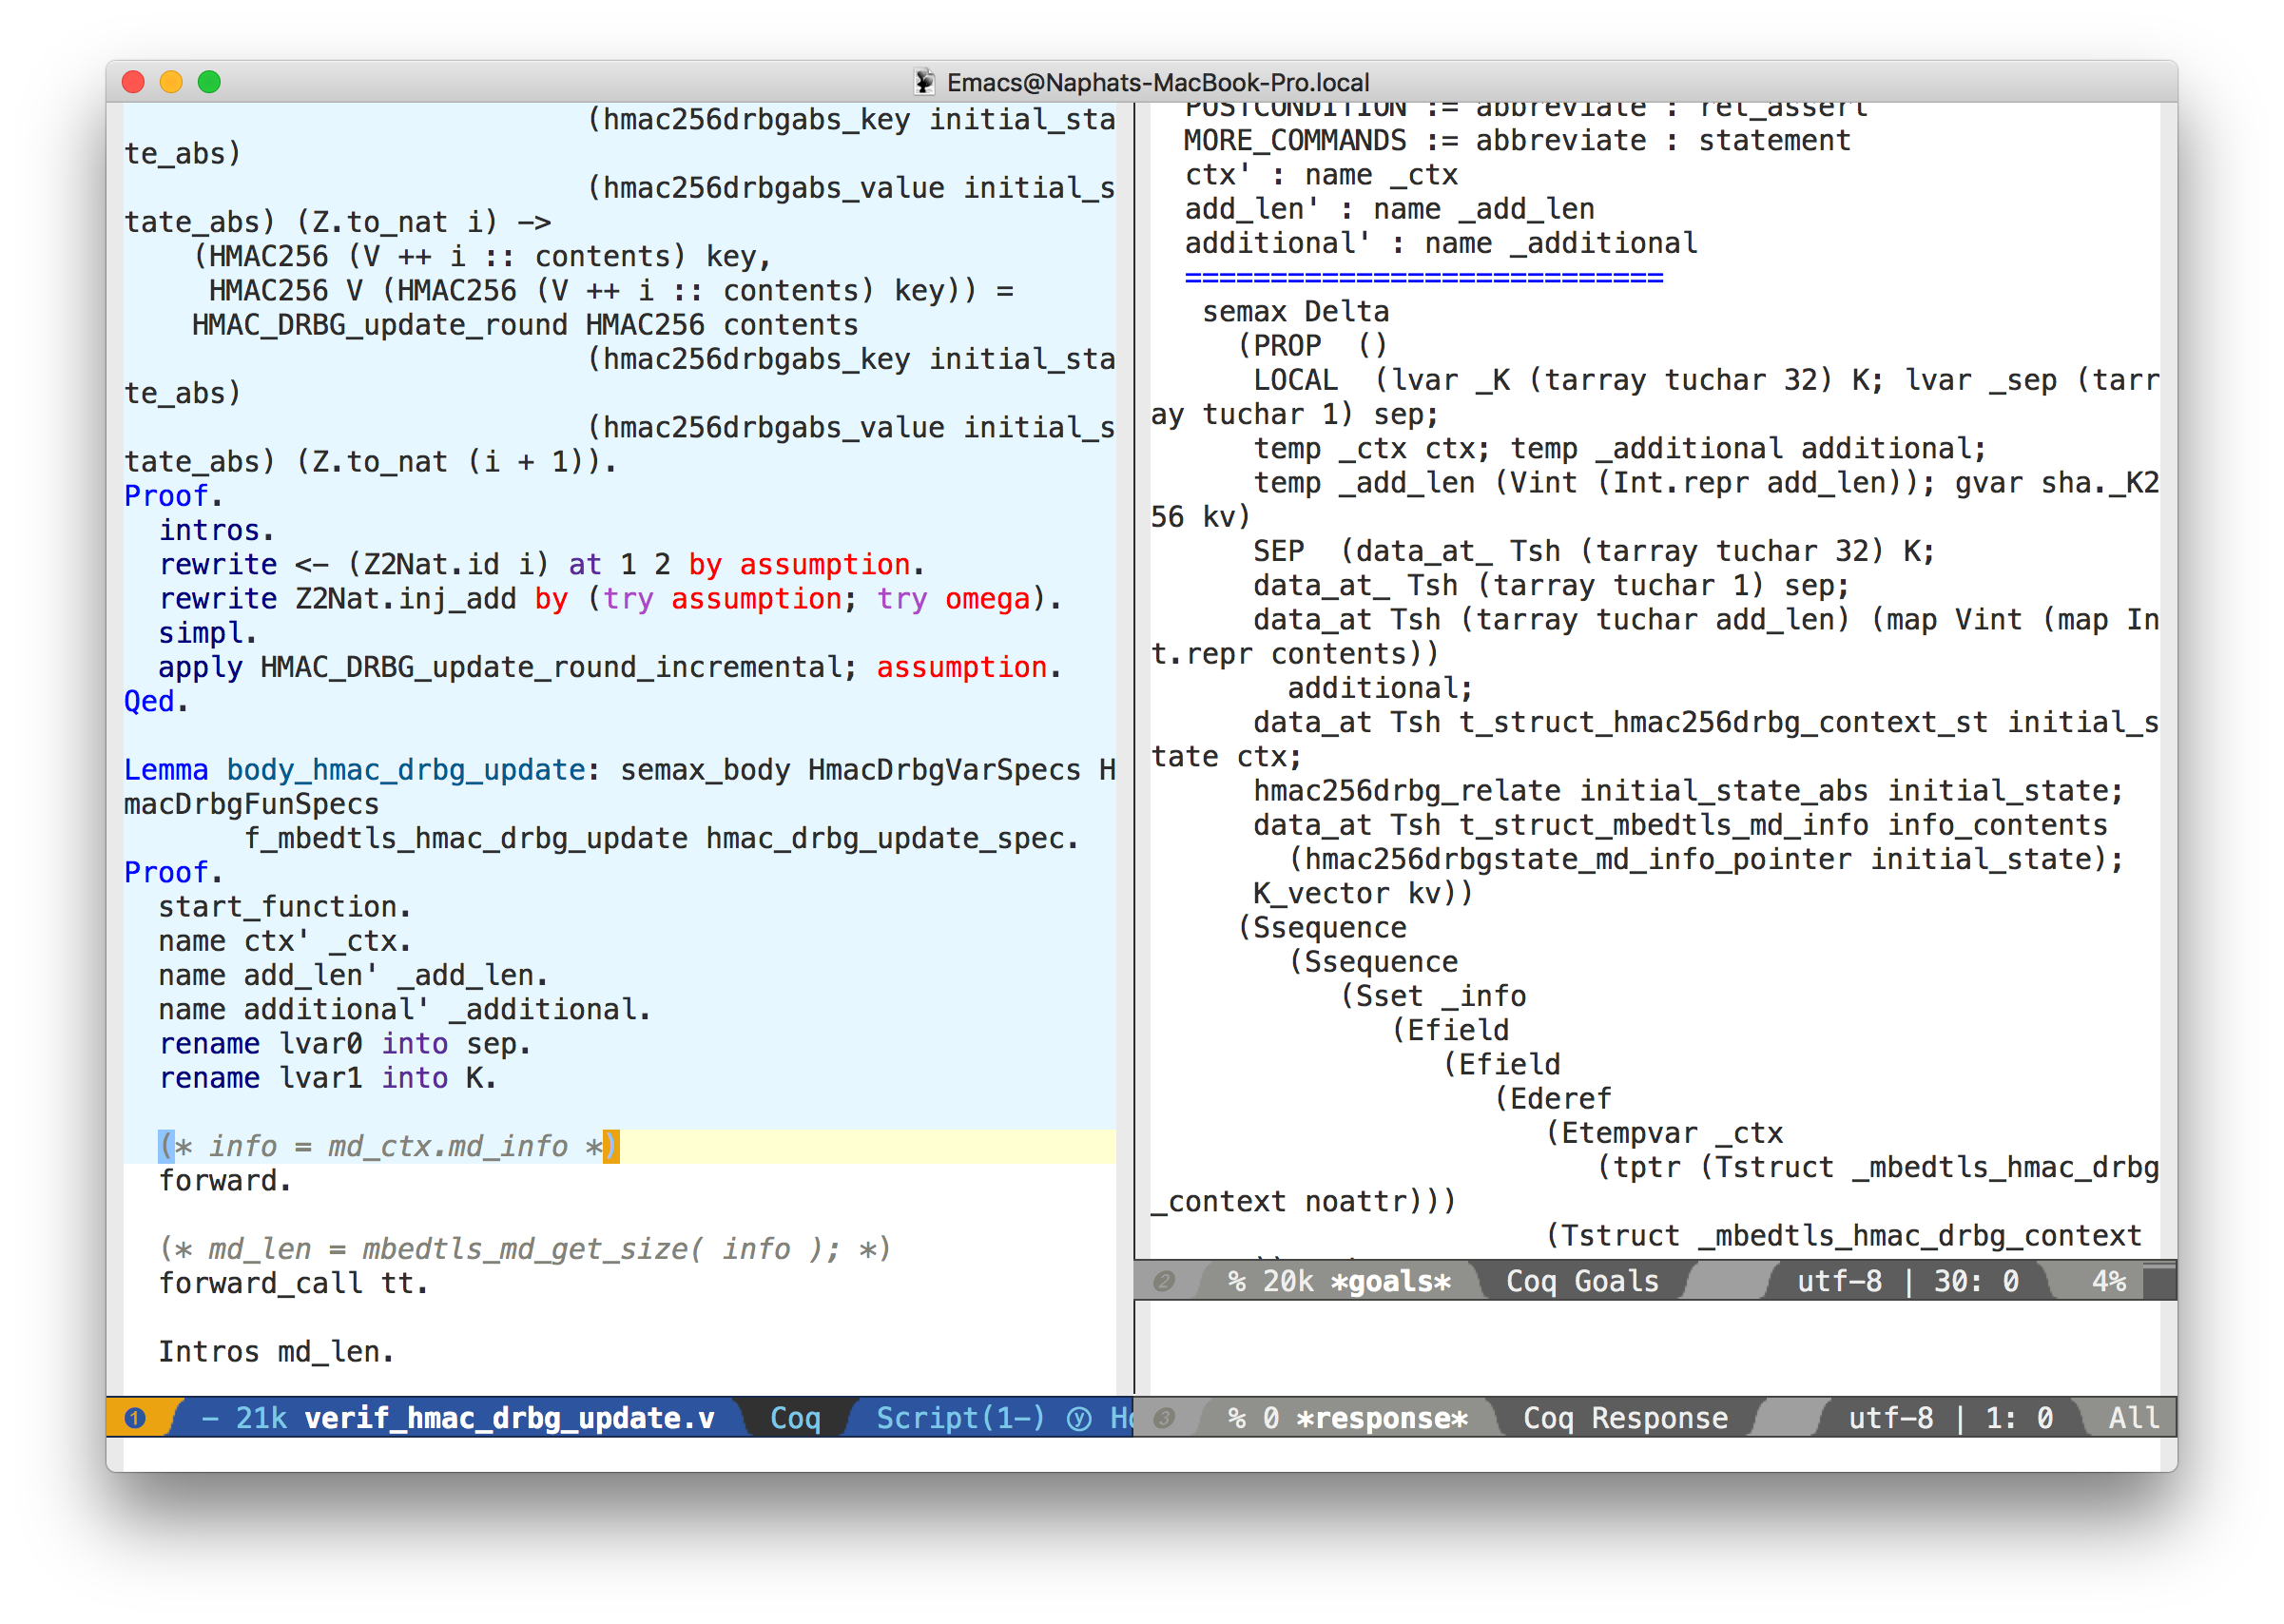
\includegraphics[width=0.9\textwidth]{before_forward}
\caption{The \lstinline{update} Function Proof}
\label{figure:before_forward}
\end{figure}

Figure \ref{figure:before_forward} shows a part of the \lstinline{update} function proof. The left pane shows the actual proof, while the right pane shows the current proof goal.

On the left pane, everything highlighted in blue is the part of the proof that has been accepted by the Coq compiler as correct. Everything in white has not been accepted, and so can still be modified. Completing the proof means compiling the entire file, or turning the entire file blue.

In the current proof goal is the proof environment, of the same \lstinline{PROP() LOCAL() SEP()} form as seen previously in \S \ref{api_spec}. The proof environment contains propositional facts, facts about local variables, and facts about memory.

The current proof goal also contains the abstract syntax tree (AST) of the C code. Each statement in the AST modifies the proof environment, and each step in the proof (left pane) is an instruction to Coq on how to step through the AST. For simple statements, such as an assignment statement, the proof automation system can figure out how the proof environment will be affected by stepping through the statement. Other statements require the proof to explicitly state how the proof environment will be affected. These statements include the \lstinline{if} statement or different kinds of loops.

Figure \ref{figure:before_forward} shows the case where the next statement in the AST is an assignment statement. This is the simple case, and so the proof command \lstinline{forward} can automatically figure out how the environment will be modified. Figure \ref{figure:after_forward} shows the same proof after the \lstinline{forward} command has been accepted by the Coq compiler. Notice the proof environment has changed in the \lstinline{LOCAL} part, and the AST no longer shows the assignment statement as the next statement.

\begin{figure}[h]
\centering
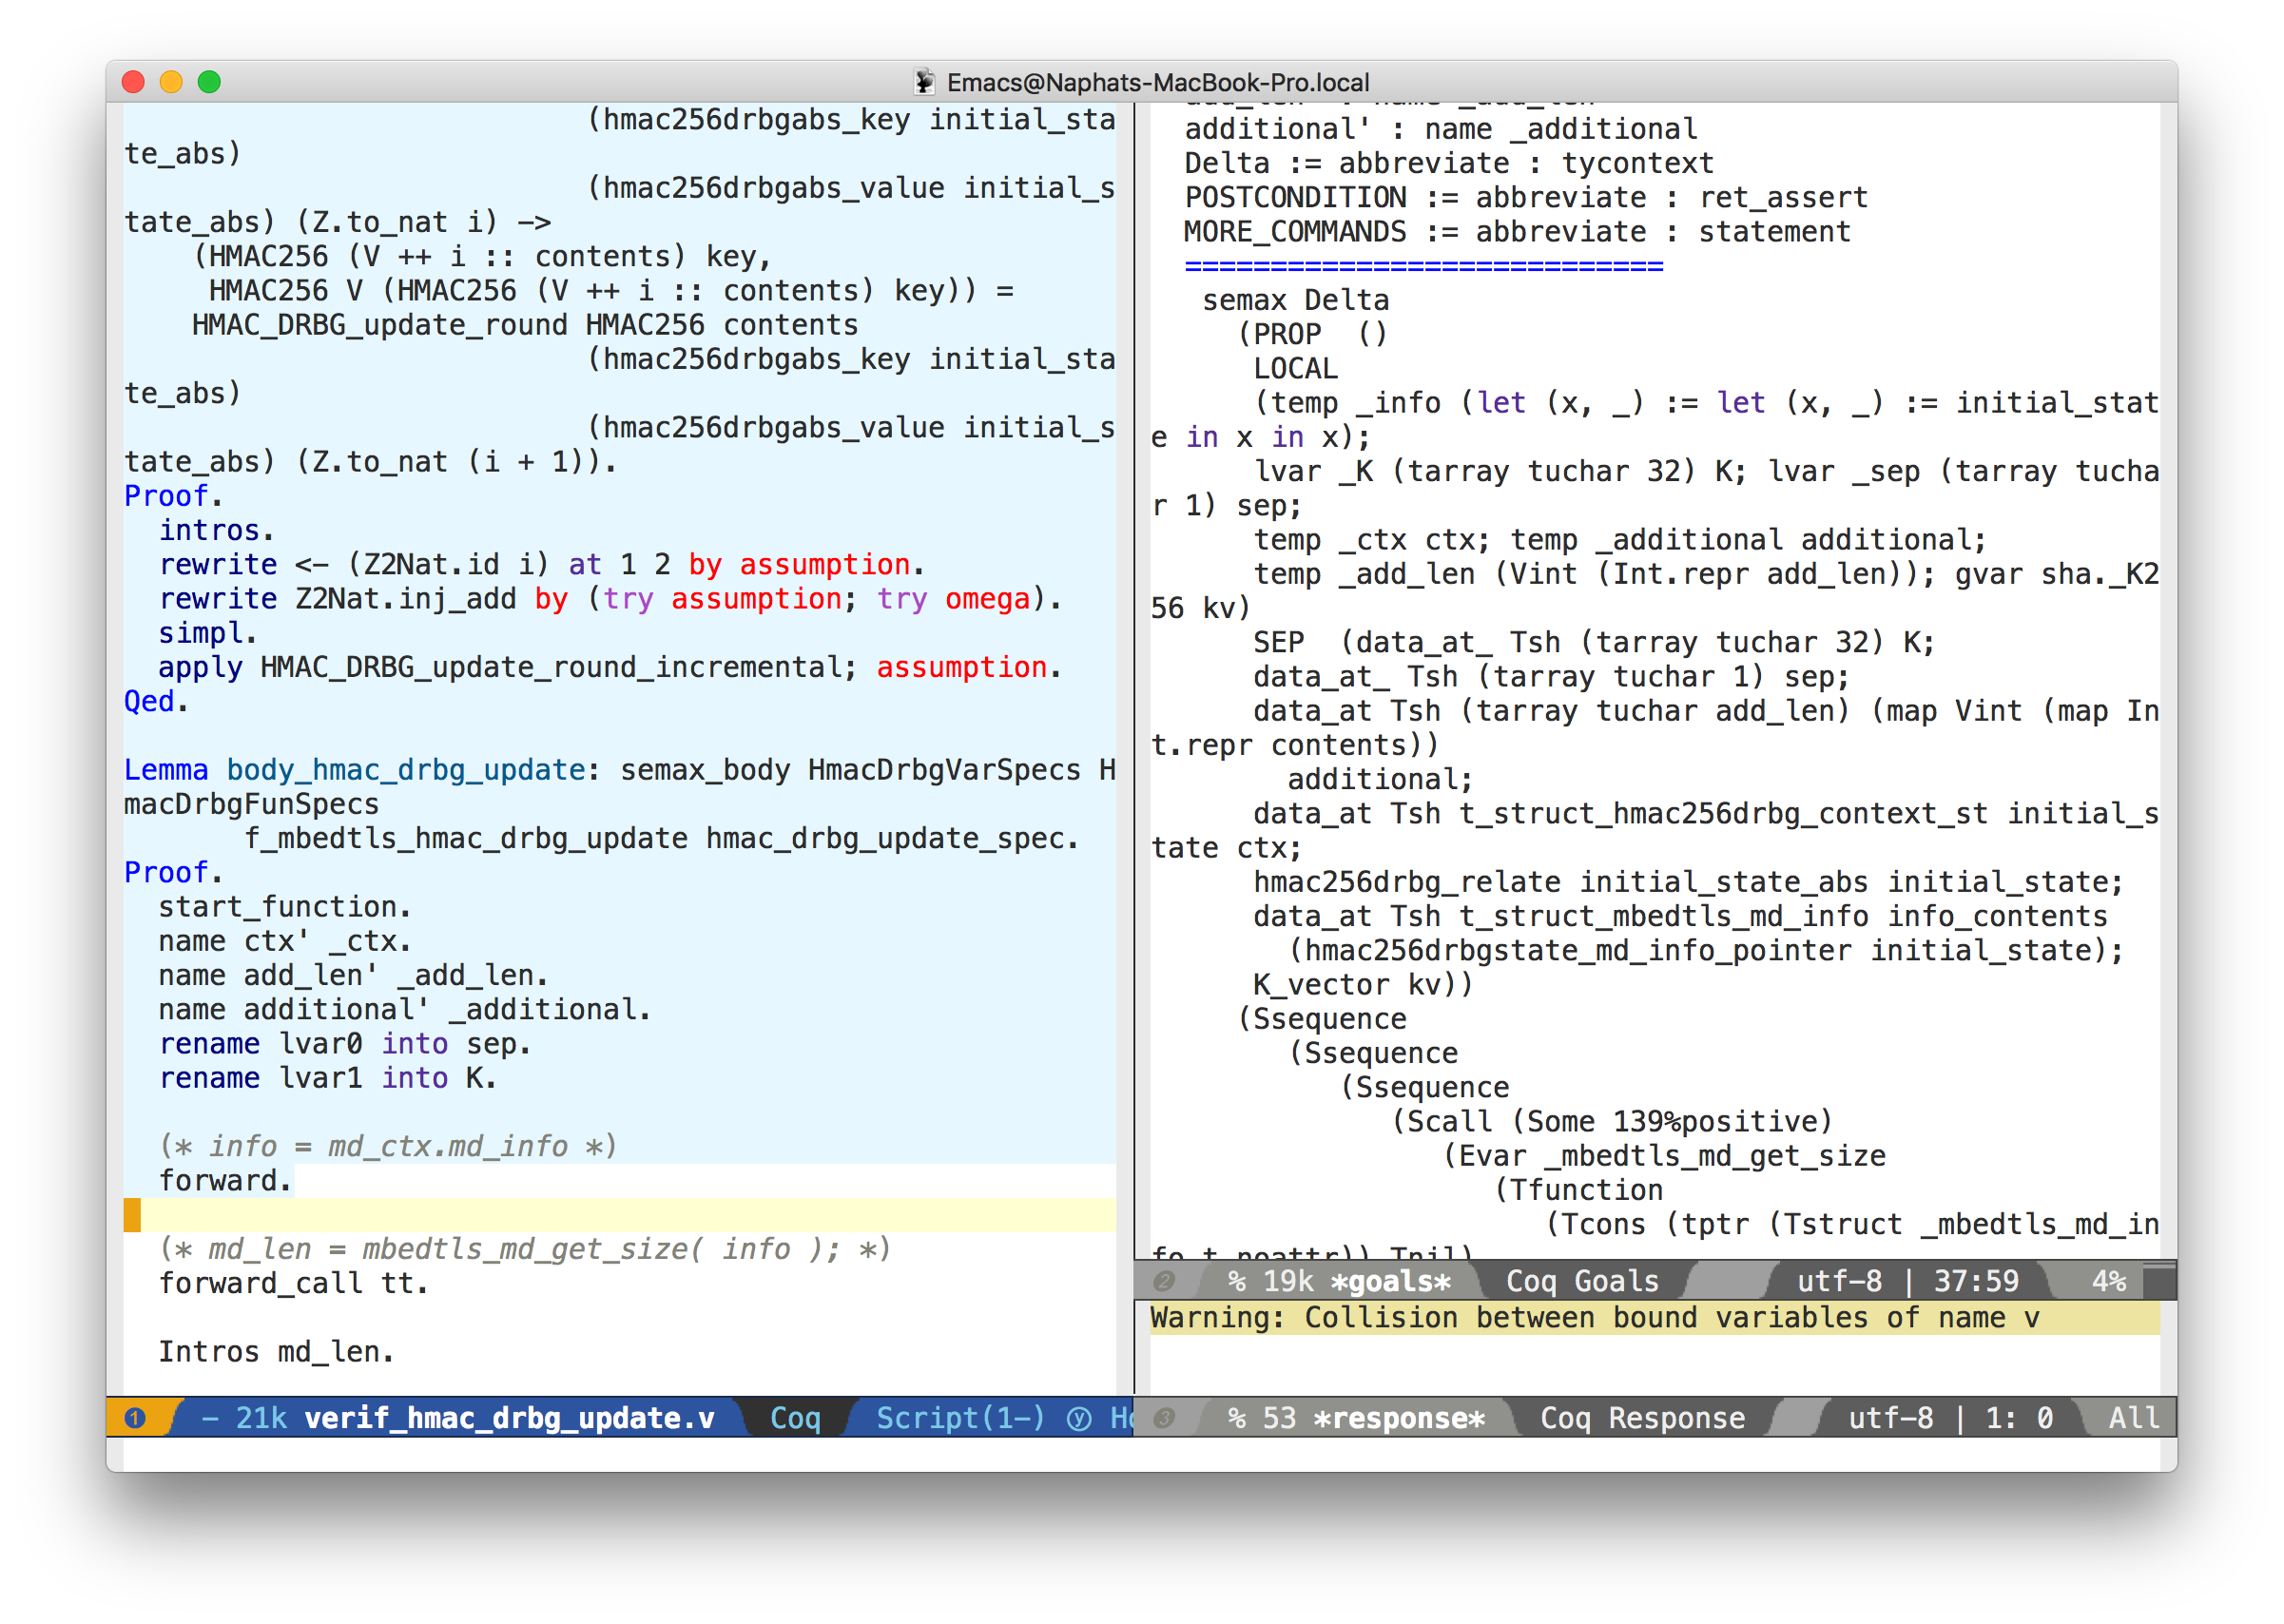
\includegraphics[width=0.9\textwidth]{after_forward}
\caption{After Compiling the \lstinline{forward} Command}
\label{figure:after_forward}
\end{figure}

The proof environment is initialized to the function preconditions. A complete proof shows that, after the entire AST has been stepped through, the modified environment implies the function postconditions. Figure \ref{figure:qed} shows when the entire proof has been compiled. Stepping through the \lstinline{Qed} command will complete the proof.

\begin{figure}[h]
\centering
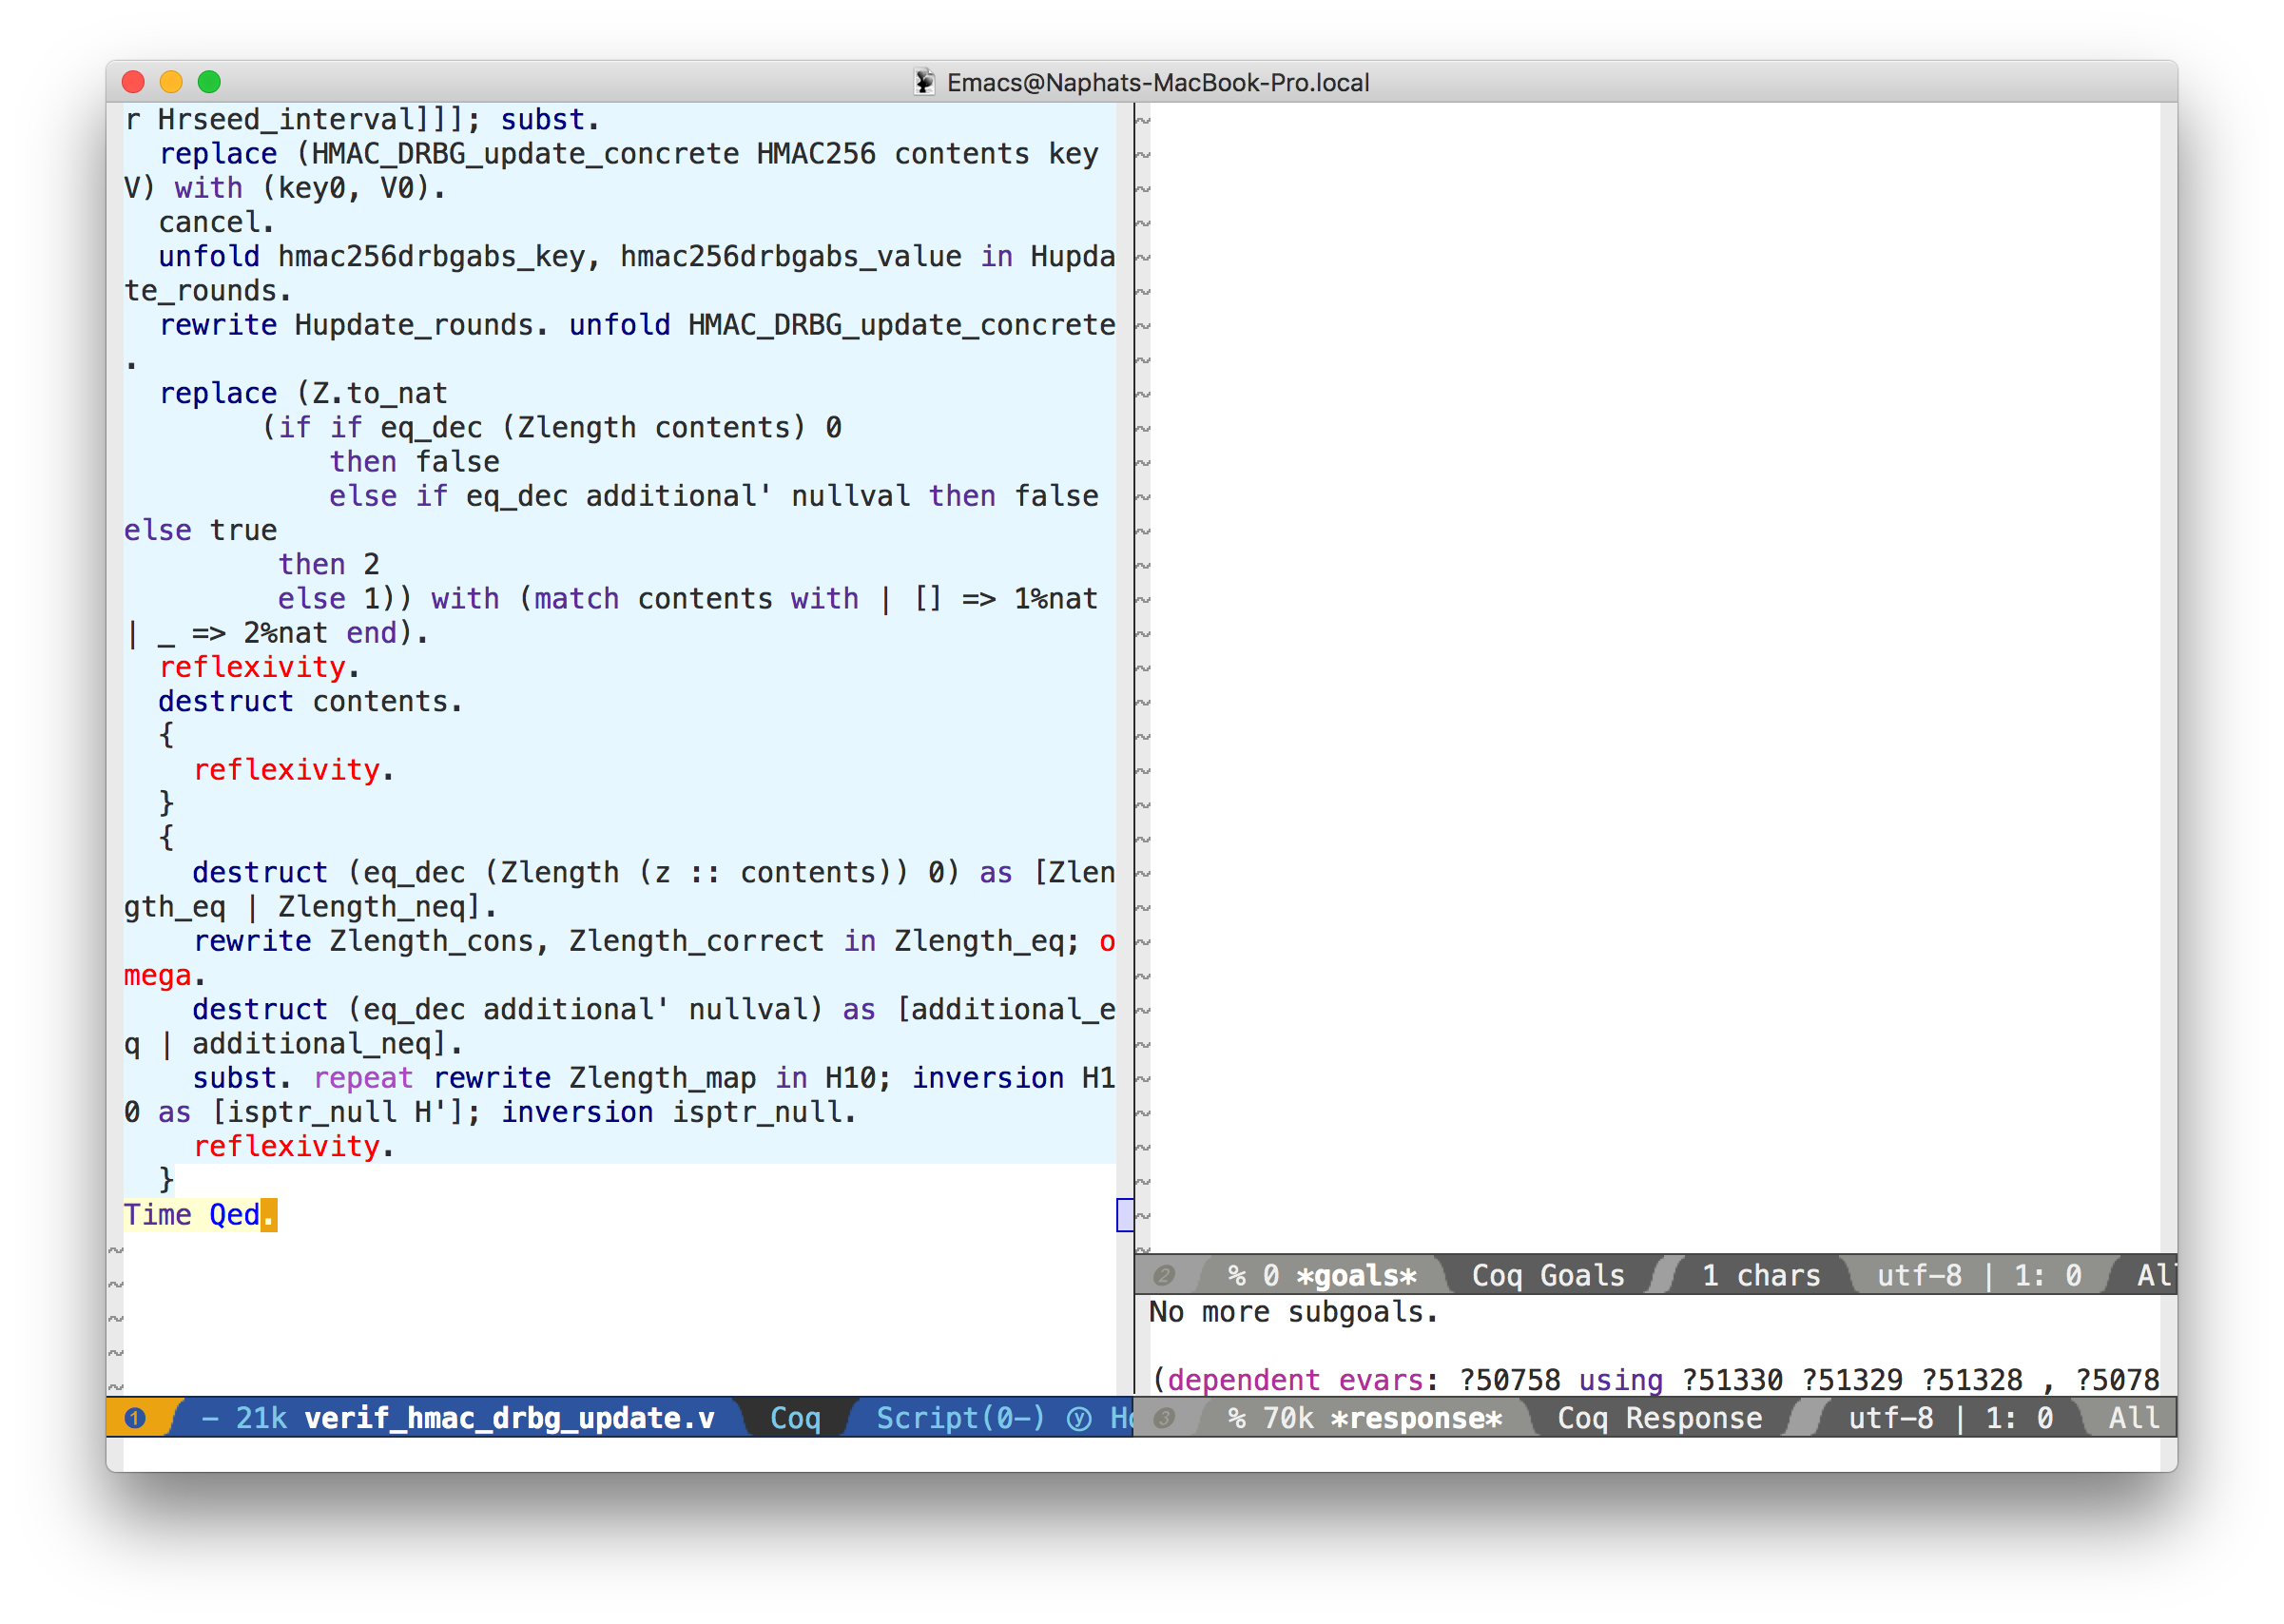
\includegraphics[width=0.9\textwidth]{qed}
\caption{At the End of the \lstinline{update} Proof}
\label{figure:qed}
\end{figure}

\subsection{Verification Statistics}

I verified the \stdtitle{mbedTLS} implementations of \lstinline{update}, \lstinline{reseed}, and \lstinline{generate} correct with respect to their API specifications. In this section, I will provide some statistics about the verifications.

\begin{table}[h!]
  \centering
  \begin{tabular}{|l|l|l|l|l|}
    \hline
    \textbf{Function} & \textbf{C (lines)} & \textbf{API Spec. (lines)} & \textbf{Proof (lines)} & \textbf{Proof (compilation time)}\\
    \hline
    \hline
    \lstinline{update} & 32 & 32 & 552 & 28 minutes \\
    \hline
    \lstinline{reseed} & 41 & 38 & 710 & 18 minutes \\
    \hline
    \lstinline{generate} & 69 & 48 & 2456 & 35 minutes \\
    \hline
  \end{tabular}
  \caption{Verification Statistics}
  \label{table:stats}
\end{table}

Line counts here include empty lines as well as comments. The compilation time was measured on a Macbook Pro with Intel Core i7, 2.5 GHz, 16 gigabytes of memory.

The actual verifications are significantly longer than the C counterpart. Fortunately, they are machine-checked, and as long as they compile successfully, it is unlikely that clients of my project would need to take a look at the actual verifications. Instead, the API specifications will be of more interest to potential clients.

\section{Difficulties}

One of the goals of my project is to serve as a bleeding-edge adopter of the VST framework and the HMAC API specification. As is the nature of bleeding-edge adoption, I encountered many difficulties, such as proof tactics failing silently and Verifiable C's theory of pointer comparisons being too weak. These difficulties were fixed as they got reported back to the developers of VST. In this section, I highlight one particular difficulty with the HMAC API specification.


\subsection{HMAC API Specification} \label{oldhmac}

The C (\stdtitle{OpenSSL}) implementation of SHA-256 HMAC defines the HMAC context as a struct with three SHA-256 contexts. The original API specification of HMAC \cite{hmac} uses this same representation as the abstract state of HMAC.

\begin{lstlisting}
    Inductive hmacabs :=
       HMACabs: forall (ctx iSha oSha: s256abs) hmacabs.
\end{lstlisting}

This representation works in the sense that the verification of the \stdtitle{OpenSSL} functions went through. Unfortunately, for clients of this API specification, this representation is often not good enough. The biggest issue is that this representation is too low-level; it does not keep track of the key. Upon being notified of this issue, the developers of the HMAC API specification were quickly able to provide a more abstract representation of the HMAC state, leading to the state machine representation shown earlier in \S \ref{hmac_interface}. The core of the verification code did not need to be changed, with some book-keeping added at the ends of translate between the new, more abstract representation to the more low-level implementation. While this issue was easily fixed, it would have been very hard to discover this issue without actually being clients of the API specification. This highlights the importance of having being the first client of the HMAC API specification.


\section{Conclusion}

I verified the \stdtitle{mbedTLS} implementations of HMAC DRBG \lstinline{update}, \lstinline{reseed}, and \lstinline{generate}. I wrote functional specifications of these functions, describing mathematically what the functions do as functional programs. Using the functional specifications, I wrote the API specifications to describe how C implementations of these functions are required to interact with local variables and memory. I then verified the \stdtitle{mbedTLS} implementations correct with respect to the API specifications. While the verifications themselves were long and unwieldy, they are machine-checked and so are not part of the code that needs to be trusted. While the functional specifications must still be trusted, they will not have to be once Katherine Ye’s parallel project on proving cryptographic properties of the functional specifications complete in the spring of 2016. Along the way, I identified some issues with the VST framework and the HMAC API specifications, and those issues are now fixed by the relevant parties. My project, along with the verification of the HMAC DRBG \lstinline{instantiate} function, will serve as one of the building blocks that future verification tasks can use.

\bstctlcite{bstctl:etal, bstctl:nodash, bstctl:simpurl}
\bibliographystyle{IEEEtranS}
\bibliography{references}

\clearpage
\appendix
\appendixpage
\section{Bridging OpenSSL’s HMAC with mbedTLS’s Message Digest Interface} \label{appendix_hmac}

As previously mentioned in \S \ref{hmac_interface}, previous verification efforts on HMAC and SHA are done on \stdtitle{OpenSSL}. Therefore, the \stdtitle{mbedTLS} DRBG implementation must somehow call into the \stdtitle{OpenSSL} HMAC implementation, so that the API specifications for HMAC can be used. To do this, I wrote a thin wrapper around the \stdtitle{mbedTLS} message digest interface. In this section, I show exactly how I did that.

The \stdtitle{mbedTLS} message digest interface declares the following functions:

\begin{lstlisting}[language=C]
    int mbedtls_md_setup( mbedtls_md_context_t *ctx, const mbedtls_md_info_t *md_info, int hmac );

    void mbedtls_md_free( mbedtls_md_context_t *ctx );

    unsigned char mbedtls_md_get_size( const mbedtls_md_info_t *md_info );

    int mbedtls_md_hmac_starts( mbedtls_md_context_t *ctx, const unsigned char *key, size_t keylen );

    int mbedtls_md_hmac_update( mbedtls_md_context_t *ctx, const unsigned char *input, size_t ilen );

    int mbedtls_md_hmac_finish( mbedtls_md_context_t *ctx, unsigned char *output);

    int mbedtls_md_hmac_reset( mbedtls_md_context_t *ctx );
\end{lstlisting}

\subsection{The HMAC Context}

In order for clients of the \stdtitle{mbedTLS} message digest interface to use \stdtitle{OpenSSL} HMAC implementation, the clients must somehow have access to \stdtitle{OpenSSL} HMAC context. The clients already have access to the \stdtitle{mbedTLS} message digest context, which is defined as the following struct:

\begin{lstlisting}[language=C]
    typedef struct mbedtls_md_context_t {
        const mbedtls_md_info_t *md_info;
        void *md_ctx;
        void *hmac_ctx;
    } mbedtls_md_context_t;
\end{lstlisting}

The \lstinline{md_info} field can mostly be ignored, as it is used to differentiate between the different types of message digest, and in this case, we are specializing the message digest to use HMAC and SHA-256. In order for clients of the message digest interface to have access to the \stdtitle{OpenSSL} HMAC context, I chose to have the \lstinline{hmac_ctx} pointer point to the \stdtitle{OpenSSL} HMAC context. This initialization happens in the \lstinline{mbedtls_md_setup} function:

\begin{lstlisting}[language=C]
    int mbedtls_md_setup( mbedtls_md_context_t *ctx, const mbedtls_md_info_t *md_info, int hmac ) {
        HMAC_CTX * sha_ctx = (HMAC_CTX *) malloc(sizeof(HMAC_CTX));
        if (sha_ctx == NULL) {
            return MBEDTLS_ERR_MD_ALLOC_FAILED;
        }
        ctx->hmac_ctx = sha_ctx;
        return 0;
    }
\end{lstlisting}

The corresponding \lstinline{mbedtls_md_free} function is done in an obvious way:

\begin{lstlisting}[language=C]
    void mbedtls_md_free( mbedtls_md_context_t *ctx ) {
        HMAC_CTX * hmac_ctx = ctx->hmac_ctx;
        free(hmac_ctx);
    }
\end{lstlisting}


\subsection{Other Functions}

The function \lstinline{mbedtls_md_get_size} can be specialized to ignore \lstinline{md_info} and always return the length of the output of SHA-256 HMAC, which is 32 bytes.

\begin{lstlisting}[language=C]
    unsigned char mbedtls_md_get_size( const mbedtls_md_info_t *md_info ) {
        return SHA256_DIGEST_LENGTH;
    }
\end{lstlisting}

The functions \lstinline{mbedtls_md_hmac_starts}, \lstinline{mbedtls_md_hmac_update}, and\\ \lstinline{mbedtls_md_hmac_finish} have counterparts in the \stdtitle{OpenSSL} library, and so can just call through to them.

\begin{lstlisting}[language=C]
    int mbedtls_md_hmac_starts( mbedtls_md_context_t *ctx, const unsigned char *key, size_t keylen ) {
        HMAC_CTX * hmac_ctx = ctx->hmac_ctx;
        HMAC_Init(hmac_ctx, (unsigned char*) key, keylen);
        return 0;
    }

    int mbedtls_md_hmac_update( mbedtls_md_context_t *ctx, const unsigned char *input, size_t ilen ) {
        HMAC_CTX * hmac_ctx = ctx->hmac_ctx;
        HMAC_Update(hmac_ctx, (const void *) input, ilen);
        return 0;
    }

    int mbedtls_md_hmac_finish( mbedtls_md_context_t *ctx, unsigned char *output) {
        HMAC_CTX * hmac_ctx = ctx->hmac_ctx;
        HMAC_Final(hmac_ctx, output);
        return 0;
    }
\end{lstlisting}

\stdtitle{OpenSSL} does not have an explicit \lstinline{reset} function. Recall that the \lstinline{reset} function takes a HMAC context \lstinline{FULL key} and takes it to \lstinline{REP key []}. That is, it makes the HMAC context ready for digesting data with the pre-existing key. In OpenSSL, this is done by passing \lstinline{NULL} as the key to \lstinline{HMAC_Init}.

\begin{lstlisting}[language=C]
    int mbedtls_md_hmac_reset( mbedtls_md_context_t *ctx ) {
        HMAC_CTX * hmac_ctx = ctx->hmac_ctx;
        HMAC_Init(hmac_ctx, NULL, SHA256_DIGEST_LENGTH);
        return 0;
    }
\end{lstlisting}
\section{DRBG API Specifications} \label{appendix_api}
In this section, I present a detailed description of the API specifications for the following functions: \lstinline{update}, \lstinline{reseed}, and \lstinline{generate}.

\subsection{The Update Function}

The API specification is as follows:

\begin{lstlisting}
    Definition hmac_drbg_update_spec :=
      DECLARE _mbedtls_hmac_drbg_update
       WITH contents: list Z,
            additional: val, add_len: Z,
            ctx: val, initial_state: hmac256drbgstate,
            initial_state_abs: hmac256drbgabs,
            kv: val, info_contents: md_info_state
        PRE [ _ctx OF (tptr t_struct_hmac256drbg_context_st), _additional OF (tptr tuchar), _add_len OF tuint ]
           PROP (
             0 <= add_len <= Int.max_unsigned;
             Zlength (hmac256drbgabs_value initial_state_abs) = Z.of_nat SHA256.DigestLength;
             add_len = Zlength contents;
             Forall isbyteZ (hmac256drbgabs_value initial_state_abs);
             Forall isbyteZ contents
           )
           LOCAL (temp _ctx ctx; temp _additional additional; temp _add_len (Vint (Int.repr add_len)); gvar sha._K256 kv)
           SEP (
             (data_at Tsh (tarray tuchar add_len) (map Vint (map Int.repr contents)) additional);
             (data_at Tsh t_struct_hmac256drbg_context_st initial_state ctx);
             (hmac256drbg_relate initial_state_abs initial_state);
             (data_at Tsh t_struct_mbedtls_md_info info_contents (hmac256drbgstate_md_info_pointer initial_state));
             (K_vector kv)
               )
        POST [ tvoid ]
           PROP ()
           LOCAL ()
           SEP (
             (hmac256drbgabs_common_mpreds (hmac256drbgabs_hmac_drbg_update initial_state_abs contents) initial_state ctx info_contents);
             (data_at Tsh (tarray tuchar add_len) (map Vint (map Int.repr contents)) additional);
             (K_vector kv)
           ).
\end{lstlisting}


The first \lstinline{WITH} variable is \lstinline{contents}, which is mathematical representation of the sequence of bytes to be consumed by the update function (\lstinline{provided_data} in the functional specification). The next two \lstinline{WITH} values are the pointer value, \lstinline{additional}, at which \lstinline{contents} is located in memory, and the length of \lstinline{contents}, \lstinline{add_len}. In the \lstinline{PROP} part of the specification, \lstinline{add_len} is restricted to be a valid unsigned integer, and the length of \lstinline{contents} is enforced to be \lstinline{add_len}. The mathematical integers in \lstinline{contents} are also enforced to be valid bytes. In the \lstinline{SEP} part, \lstinline{additional} is said to point to \lstinline{contents}. In the postcondition, the same \lstinline{SEP} clause appears, showing that the update function does not change the memory pointed to by \lstinline{additional}.

The next \lstinline{WITH} value is the pointer value, \lstinline{ctx}, pointing to the DRBG struct. The next two \lstinline{WITH} values are the abstract and concrete DRBG states, respectively. The last \lstinline{WITH} value is the content of the struct denoting what kind of HMAC is being used, \lstinline{info_contents}. In the \lstinline{PROP} clause, the sequence \lstinline{V} part of the abstract state is enforced to be the size of the output of the HMAC function and enforced to contain valid bytes. This is an invariant that the update function and all public functions enforce, and so will be seen throughout all API specifications. In the \lstinline{SEP} clause, \lstinline{ctx} is said to point to an area in memory that contains the concrete state, and the concrete state is related to the abstract state by the equivalence definition. The info pointer from the concrete state also points to a valid address containing \lstinline{info_contents}. In the post condition, there is a new abstract state calculated by \lstinline{hmac256drbgabs_hmac_drbg_update}, which is just a wrapper around the functional specification with the HMAC256 function used. In the \lstinline{SEP} part, there exists a corresponding concrete state pointed to by \lstinline{ctx} that is equivalent to the new abstract state. This new concrete state’s info pointer also points to the same valid memory location containing \lstinline{info_contents}. This is what the definition \lstinline{hmac256drbgabs_common_mpreds} encapsulates.

The \lstinline{WITH} value \lstinline{kv} represents the pointer value to the SHA K vector, which is a global constant array in the SHA-256 implementation. For more information, see the verification of SHA-256 \cite{sha}.

\subsection{The Reseed Function}

The API specification for the \lstinline{reseed} function is as follows:

\begin{lstlisting}
    Definition hmac_drbg_reseed_spec :=
      DECLARE _mbedtls_hmac_drbg_reseed
       WITH contents: list Z,
            additional: val, add_len: Z,
            ctx: val, initial_state: hmac256drbgstate,
            initial_state_abs: hmac256drbgabs,
            kv: val, info_contents: md_info_state,
            s: ENTROPY.stream
        PRE [ _ctx OF (tptr t_struct_hmac256drbg_context_st), _additional OF (tptr tuchar), _len OF tuint ]
           PROP (
             0 <= add_len <= Int.max_unsigned;
             Zlength (hmac256drbgabs_value initial_state_abs) = Z.of_nat SHA256.DigestLength;
             add_len = Zlength contents;
             hmac256drbgabs_entropy_len initial_state_abs = 32;
             Forall isbyteZ (hmac256drbgabs_value initial_state_abs);
             Forall isbyteZ contents
           )
           LOCAL (temp _ctx ctx; temp _additional additional; temp _len (Vint (Int.repr add_len)); gvar sha._K256 kv)
           SEP (
             (data_at Tsh (tarray tuchar add_len) (map Vint (map Int.repr contents)) additional);
             (data_at Tsh t_struct_hmac256drbg_context_st initial_state ctx);
             (hmac256drbg_relate initial_state_abs initial_state);
             (data_at Tsh t_struct_mbedtls_md_info info_contents (hmac256drbgstate_md_info_pointer initial_state));
             (Stream s);
             (K_vector kv)
               )
        POST [ tint ]
           EX ret_value:_,
           PROP (
               return_value_relate_result (mbedtls_HMAC256_DRBG_reseed_function s initial_state_abs contents) ret_value
             )
           LOCAL (temp ret_temp ret_value)**
           SEP (
             (hmac256drbgabs_common_mpreds (hmac256drbgabs_reseed initial_state_abs s contents) initial_state ctx info_contents);
             (data_at Tsh (tarray tuchar add_len) (map Vint (map Int.repr contents)) additional);
             (Stream (get_stream_result (mbedtls_HMAC256_DRBG_reseed_function s initial_state_abs contents)));
             (K_vector kv)
           ).
\end{lstlisting}

Notice a new notation here: \lstinline{EX ret_value:_}. This can be read literally as “there exists a variable \lstinline{ret_value} that satisfies the postcondition”. This existential variable captures the return value of the function, and its value is enforced in the \lstinline{PROP} part of the postcondition. The return value is enforced to be 0 if the reseed succeeds, a specific nonzero value if the reseed fails because of a failure to get entropy, and any nonzero value if the reseed fails for any other reason.

\lstinline{mbedtls_HMAC256_DRBG_reseed_function} is just a wrapper around the functional specification of the reseed function, with the reseed algorithm and other dependencies filled in. \lstinline{hmac256drbgabs_reseed} returns the resulting abstract state from the reseed function if the reseed succeeds, or the initial abstract state otherwise.

Much like the \lstinline{update} function, the first three \lstinline{WITH} values are used for the additional data parameter. \lstinline{additional} is a pointer value that points to \lstinline{contents}, of length \lstinline{add_len}, and the function leaves this relation untouched.

Again, much like the \lstinline{update} function, the next three \lstinline{WITH} values are the pointer value to the DRBG state, the abstract DRBG state, and the concrete DRBG state. The only new property is in the \lstinline{PROP} part of the precondition, requiring the \lstinline{entropy_len} component to be 32. In \stdtitle{NIST SP 800-90A} and therefore in the functional specification, this is a global, fixed constant, but \stdtitle{mbedTLS} varies this value based on the type of HMAC used and fixes the value upon instantiation. With HMAC256, this is fixed to be 32.

Unlike the \lstinline{update} function, the \lstinline{reseed} function needs to reason about entropy; that is the whole point of reseeding! The \lstinline{WITH} value \lstinline{s} represents the entropy stream to be used, and a new one is passed back out in the \lstinline{SEP} part of the postcondition.

\subsection{The Generate Function}

The API specification for the \lstinline{generate} function is as follows:

\begin{lstlisting}
    Definition hmac_drbg_generate_spec :=
      DECLARE _mbedtls_hmac_drbg_random_with_add
       WITH contents: list Z,
            additional: val, add_len: Z,
            output: val, out_len: Z,
            ctx: val, initial_state: hmac256drbgstate,
            initial_state_abs: hmac256drbgabs,
            kv: val, info_contents: md_info_state,
            s: ENTROPY.stream
        PRE [ _p_rng OF (tptr tvoid), _output OF (tptr tuchar), _out_len OF tuint, _additional OF (tptr tuchar), _add_len OF tuint ]
           PROP (
             0 <= add_len <= Int.max_unsigned;
             0 <= out_len <= Int.max_unsigned;
             Zlength (hmac256drbgabs_value initial_state_abs) = Z.of_nat SHA256.DigestLength;
             add_len = Zlength contents;
             hmac256drbgabs_entropy_len initial_state_abs = 32;
             hmac256drbgabs_reseed_interval initial_state_abs = 10000;
             0 <= hmac256drbgabs_reseed_counter initial_state_abs <= Int.max_signed;
             Forall isbyteZ (hmac256drbgabs_value initial_state_abs);
             Forall isbyteZ contents
           )
           LOCAL (temp _p_rng ctx; temp _output output; temp _out_len (Vint (Int.repr out_len)); temp _additional additional; temp _add_len (Vint (Int.repr add_len)); gvar sha._K256 kv)
           SEP (
             (data_at_ Tsh (tarray tuchar out_len) output);
             (data_at Tsh (tarray tuchar add_len) (map Vint (map Int.repr contents)) additional);
             (data_at Tsh t_struct_hmac256drbg_context_st initial_state ctx);
             (hmac256drbg_relate initial_state_abs initial_state);
             (data_at Tsh t_struct_mbedtls_md_info info_contents (hmac256drbgstate_md_info_pointer initial_state));
             (Stream s);
             (K_vector kv)
               )
        POST [ tint ]
           EX ret_value:_,
           PROP (
               return_value_relate_result (mbedtls_HMAC256_DRBG_generate_function s initial_state_abs out_len contents) ret_value
             )
           LOCAL (temp ret_temp ret_value)
           SEP (
             (match mbedtls_HMAC256_DRBG_generate_function s initial_state_abs out_len contents with
                | ENTROPY.error _ _ => (data_at_ Tsh (tarray tuchar out_len) output)
                | ENTROPY.success (bytes, _) _ => (data_at Tsh (tarray tuchar out_len) (map Vint (map Int.repr bytes)) output)
              end
             );
             (hmac256drbgabs_common_mpreds (hmac256drbgabs_generate initial_state_abs s out_len contents) initial_state ctx info_contents);
             (data_at Tsh (tarray tuchar add_len) (map Vint (map Int.repr contents)) additional);
             (Stream (get_stream_result (mbedtls_HMAC256_DRBG_generate_function s initial_state_abs out_len contents)));
             (K_vector kv)
           ).
\end{lstlisting}

The main difference between this specification and the API specification of \lstinline{reseed} is that the generate function takes as input a pointer (\lstinline{output}) to a buffer of size \lstinline{out_len}, which is filled with the resulting stream of bytes on success and left alone on failure.

\end{document}
